\documentclass{report}

\usepackage[warn]{mathtext}
\usepackage[T2A]{fontenc}
\usepackage[utf8]{luainputenc}
\usepackage[english, russian]{babel}
\usepackage[pdfpagemode=UseNone,colorlinks,allcolors=black]{hyperref}
\usepackage{tempora}
\usepackage[12pt]{extsizes}
\usepackage{listings}
\usepackage{color}
\usepackage{geometry}
\usepackage{enumitem}
\usepackage{multirow}
\usepackage{graphicx}
\usepackage{indentfirst}
\usepackage{amsmath}
\usepackage{soul}

\graphicspath{ {../../modules/task_1/shelepin_n_trapezoidal_rule/images/} }
\sethlcolor{gray}

\geometry{a4paper,top=2cm,bottom=2cm,left=2.5cm,right=1.5cm}
\setlength{\parskip}{0.5cm}
\setlist{nolistsep, itemsep=0.3cm,parsep=0pt}

\usepackage{listings}
\lstset{language=C++,
        basicstyle=\footnotesize,
		keywordstyle=\color{blue}\ttfamily,
		stringstyle=\color{red}\ttfamily,
		commentstyle=\color{green}\ttfamily,
		morecomment=[l][\color{red}]{\#}, 
		tabsize=4,
		breaklines=true,
  		breakatwhitespace=true,
  		title=\lstname,       
}

\makeatletter
\renewcommand\@biblabel[1]{#1.\hfil}
\makeatother

\begin{document}

\begin{titlepage}

\begin{center}
Министерство науки и высшего образования Российской Федерации
\end{center}

\begin{center}
Федеральное государственное автономное образовательное учреждение высшего образования \\
Национальный исследовательский Нижегородский государственный университет им. Н.И. Лобачевского
\end{center}

\begin{center}
Институт информационных технологий, математики и механики
\end{center}

\vspace{4em}

\begin{center}
\textbf{\LargeОтчет по лабораторной работе} \\
\end{center}
\begin{center}
\textbf{\Large«Вычисление многомерных интегралов с использованием многошаговой схемы (метод трапеций)»} \\
\end{center}

\vspace{4em}

\newbox{\lbox}
\savebox{\lbox}{\hbox{text}}
\newlength{\maxl}
\setlength{\maxl}{\wd\lbox}
\hfill\parbox{7cm}{
\hspace*{5cm}\hspace*{-5cm}\textbf{Выполнил:} \\ студент группы 381906-2 \\ Шелепин Н. А.\\
\\
\hspace*{5cm}\hspace*{-5cm}\textbf{Проверил:}\\ доцент кафедры МОСТ, \\ кандидат технических наук \\ Сысоев А. В.\\
}
\vspace{\fill}

\begin{center} Нижний Новгород \\ 2022 \end{center}

\end{titlepage}

\setcounter{page}{2}

% Содержание
\tableofcontents
\newpage

% Введение
\section*{Введение}
\addcontentsline{toc}{section}{Введение}
\parВ ряде задач возникает необходимость вычисления определенного интеграла от некоторой функции:
\begin{align*}
    I = \int_{a}^{b}f(x)\cdot dx
\end{align*}
где  – подынтегральная функция, непрерывная на отрезке $[a,b]$.
     
\par Геометрический смысл интеграла заключается в том, что если $f(x)\ge 0$ на отрезке $[a,b]$, то интеграл $\int_{a}^{b}f(x)\cdot dx$ численно равен площади фигуры, ограниченной графиком функции $y=f(x)$, отрезком оси абсцисс, прямой $x = a$ и прямой $x = b$. Таким образом, вычисление интеграла равносильно вычислению площади криволинейной трапеции.

\begin{figure}[hp]
    \centering
    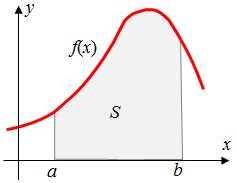
\includegraphics{graph1}
    \caption{Геометрический смысл интеграла}
\end{figure}

\par Задача численного интегрирования состоит в замене исходной подынтегральной функции некоторой аппроксимирующей функцией (обычно полиномом).
\par Численное интегрирование применяется, когда:
\begin{enumerate}
    \item Сама подынтегральная функция не задана аналитически. Например, она представлена в виде таблицы (массива) значений в узлах некоторой расчётной сетки.
    \item Аналитическое представление подынтегральной функции известно, но её первообразная не выражается через аналитические функции.
\end{enumerate}

Способы численного вычисления определенных интегралов основаны на замене интеграла конечной суммой:
\begin{align*}
    \int_{a}^{b}f(x)\cdot dx \approx \sum_{j=1}^{N}c_{j} \cdot f(x_{j})
\end{align*}

\par Одним из наиболее простых методов численного интегрирования является \textbf{метод трапеций}. Площадь криволинейной трапеции заменяется площадью многоугольника, составленного из $N$ трапеций, при этом кривая заменяется вписанной в нее ломаной. На каждом из частичных отрезков функция аппроксимируется прямой, проходящей через конечные значения, при этом площадь трапеции на каждом отрезке определяется по формуле:
\begin{align*}
    \int_{a}^{b}f(x)\cdot dx \approx \sum_{j=1}^{N} \frac{f(x_j)+f(x_{j-1})}{2}h=h\left[ \frac{1}{2}(f_1+f_N)+f_2+...+f_{N-1} \right]
\end{align*}

\begin{figure}[hp]
    \centering
    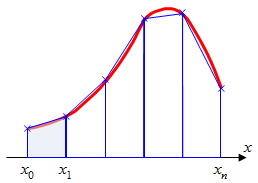
\includegraphics{graph2}
    \caption{Интегрирование методом методом трапеций}
\end{figure}

\newpage

% Постановка задачи
\section*{Постановка задачи}
\addcontentsline{toc}{section}{Постановка задачи}
\par В данном лабораторной работе требуется реализовать последовательную версию и параллельные версии алгоритма интегрирования методом трапеций, причем алгоритм должен будет уметь работать с функциями разных размерностей. Многошаговая схема здесь подразумевает постепенное вычисление интеграла. Также нужно провести вычислительные эксперименты для сравнения времени работы алгоритмов, используя при этом фрэймворк для разработки автоматических тестов Google Test, сделать выводы об эффективности реализованных алгоритмов.
\par Параллельные версии алгоритмов должны быть реализованы при помощи библиотек OpenMP, TBB и std::thread из стандартной библиотеки C++.
\newpage

% Описание алгоритма
\section*{Описание алгоритма}
\addcontentsline{toc}{section}{Описание алгоритма}
\par Алгоритм интегрирования методом трапеций для многомерных интегралов запускает цикл длины числа разбиений функции, возведенной в степень числа размерности интеграла и в своих итерациях находит все возможные точки, которые присутствуют в плоскости/объеме подынтегральной функции. От всех точек берется значение данной функции и суммируется. Затем сумма домножается на значения длин отрезков разбиения по всем размерностям, что в итоге дает нам искомую площадь/объем. Подробнее этот алгоритм выглядит следующим образом:
\begin{enumerate}
\item В цикле от 0 до значения размерности интеграла вычислить значение длины отрезка разбиения для каждой размерности и сосчитать длину общего цикла, умножив число разбиений на само себя по числу размерности, фактически возводя число разбиений в степень размерности интеграла.
\item Объявить переменную, в которую будем записывать результат, присвоить ей значение 0.
\item В цикле размером общей длины, которую мы только что вычислили:
  \begin{enumerate}
    \item Запустить цикл по размерности и посчитать значение точки на данной итерации.
    \item В переменную результата суммировать значение функции от данной точки.
  \end{enumerate}
\item В цикле по размерности домножить значение переменной результата на каждую длину отрезка разбиения.
\end{enumerate}
\newpage

% Описание схемы распараллеливания
\section*{Описание схемы распараллеливания}
\addcontentsline{toc}{section}{Описание схемы распараллеливания}
\par В нашей программе есть цикл, который вычисляет значение всех возможных точек, и содержит число итераций, равное числу разбиений в степени размерности интеграла. Этот цикл может достигать значительных размеров, и имеет смысл его распараллелить, то есть разбить на части, чтобы каждый поток вычислял своё число итераций.
\par В реализации с OpenMP мы воспользуемся директивой \emph{\#pragma omp parallel for reduction(+ : result)}, где \emph{parallel} запускает выполнение параллельного кода, \emph{for} запускает распараллеливание цикла for, а \emph{reduction(+ : result)} совершает редукцию на переменной result с операцией суммирования, что означает, что в каждом потоке создастся локальная переменная result, которые в конце всех итераций редуцируются в глобальную суммированием.
\par В реализации с TBB нам подойдет функция \emph{tbb::parallel\_reduce}, так как в конце каждой итерации мы суммируем результат в переменную result. Логика работы схожа с OpenMP, только мы вручную указываем диапазон, такой же, как у изначального цикла.
\par И, наконец, в реализации с std::thread мы действуем по следующему алгоритму:
\begin{enumerate}
    \item Вручную или автоматически, в зависимости от конфигурации системы, задаем число потоков.
    \item Создаем массив \emph{std::vector<std::thread>} для хранения потоков и массив \emph{std::vector<double>} для хранения локальных результатов.
    \item Задаем число \emph{grainsize} --- число итераций, которые выполнит каждый поток.
    \item Задаем лямбда-функцию, которую будет выполнять каждый поток. Она содержит исходный цикл, в котором начальное и конечное значения заменены на begin и end, которые функция принимает на вход. Результатов работы функции является локальный результат, который записывается в массив локальных результатов по индексу потока.
    \item В цикле по числу потоков создаем поток std::thread с указанием лямбда-функции, начала и конца, помещаем его в массив.
    \item Для последнего потока указываем конец как число итераций (поток работает "до конца").
    \item Для каждого потока из массива вызываем метод \emph{join} для синхронизации.
    \item Суммируем все локальные результаты в одну переменную и домножаем на все значения длин отрезков разбиения.
\end{enumerate}
\newpage

% Описание программной реализации
\section*{Описание программной реализации}
\addcontentsline{toc}{section}{Описание программной реализации}
Программа состоит из заголовочного файла \emph{trapezoidal\_rule.h} и двух файлов исходного кода \emph{trapezoidal\_rule.cpp} и \emph{main.cpp}.
\par В заголовочном файле находятся прототипы функций для последовательного и параллельных алгоритмов интегрирования методом трапеций.

\par Последовательная функция алгоритма интегрирования методом трапеций:
\begin{lstlisting}
double getSeqTrapezoidal(
    const int n, const std::vector<std::pair<double, double>>& limits,
    const std::function<double(std::vector<double>)>& f);
\end{lstlisting}
Параметры функции: число разбиений, массив пределов интегрирования, функция, по которой нужно интегрировать.

\par Параллельная функция алгоритма интегрирования методом трапеций (функция совпадает для всех реализаций):
\begin{lstlisting}
double getParallelTrapezoidal(
    const int n, const std::vector<std::pair<double, double>>& limits,
    const std::function<double(std::vector<double>)>& f);
\end{lstlisting}
Параметры совпадают с последовательной функцией.

\par В файле исходного кода \emph{trapezoidal\_rule.cpp} содержится реализация функций, объявленных в заголовочном файле. В файле исходного кода \emph{main.cpp} содержатся тесты для проверки корректности программы.
\newpage

% Подтверждение корректности
\section*{Подтверждение корректности}
\addcontentsline{toc}{section}{Подтверждение корректности}
\par Для подтверждения корректности работы программы на фрэймфорке Google Test были написаны 5 тестов для каждой реализации. В каждом тесте определяется своя функция для интегрирования, число разбиений и пределы интегрирования. Так же в каждом тесте записан предполагаемый результат интегрирования для сравнения.
\par В последовательной реализации в каждом тесте мы просто запускаем алгоритм и сравниваем полученный результат с контрольным. В параллельных версиях мы запускаем оба алгоритма, последовательный и параллельный, и сравниваем результат работы каждого с контрольным значением.
\newpage

% Результаты экспериментов
\section*{Результаты экспериментов}
\addcontentsline{toc}{section}{Результаты экспериментов}
Для проведения экспериментов по вычислению эффективности работы разных реализаций программы использовалась система со следующей конфигурацией:
\begin{itemize}
\item Процессор: AMD FX-8320E, 3.5 ГГц, ядер: 8, потоков: 8;
\item Оперативная память: 16 ГБ (DDR3), 1866 МГц;
\item Операционная система: Windows 10 Pro.
\end{itemize}

\par Для проведения экспериментов был создан специальный тест, который 10 раз запускает все 4 версии алгоритма, а затем усредняет полученные результаты.  
\begin{enumerate}
    \item Функция интегрирования: $\frac{sin(x) - cos(y)}{z \cdot z}$.
    \item Пределы интегрирования: $\{1, 3\}$, $\{5, 8\}$, $\{10, 12\}$.
    \item Число разбиений: 100.
    \item Число потоков: 8.
\end{enumerate}

\par Результаты экспериментов:
\begin{table}[!h]
\centering
\begin{tabular}{| c | c | c |}
\hline
Версия & Время работы (сек.) & Ускорение (раз) \\
\hline
Последовательный        & 0.916082        & -         \\
OpenMP        & 0.408438        & 2.2          \\
TBB       & 0.24093        & 3.8         \\
std::thread        & 0.561037        & 1.6           \\
\hline
\end{tabular}
\caption{Результаты экспериментов}
\end{table}

\newpage

% Выводы из результатов экспериментов
\section*{Выводы из результатов экспериментов}
\addcontentsline{toc}{section}{Выводы из результатов экспериментов}
\par Из данных, полученных в результате экспериментов (см. Таблицу 1), можно сделать вывод, что все параллельные реализации позволяют достичь ускорения по времени.
\par Версия с TBB показала наилучший результат, а версия с std::thread --- наихудший. Отличия в скорости работы OpenMP и TBB можно связать с тем, что в TBB функция \emph{parallel\_reduce} реализована эффективнее, чем редукция в OpenMP.
\par Версия с std::thread показала наихудший результат, так как в ней мы вручную создаем потоки, делим данные и используем стандартную синхронизацию \emph{join}, которая ждёт самый медленный поток. Так же эта реализация больше подвержена стандартным проблемам параллельного программирования, таким как промах по кэшу и гонка данных.
\newpage

% Заключение
\section*{Заключение}
\addcontentsline{toc}{section}{Заключение}
Таким образом, в рамках данной лабораторной работы были разработаны последовательный и три версии параллельного алгоритма интегрирования методом трапеций для многомерных интегралов. Проведенные тесты показали корректность реализованной программы, а проведенные эксперименты доказали эффективность распараллеливания этого алгоритма.
\newpage

% Литература
\section*{Литература}
\addcontentsline{toc}{section}{Литература}
\begin{enumerate}
\item IFMO - Электронный ресурс. URL: \newline \url{http://aco.ifmo.ru/el_books/numerical_methods/lectures/glava2_1.html}
\item Habr - Электронный ресурс. URL: \newline \url{https://habr.com/ru/post/479202/}
\item Educative - Электронный ресурс. URL: \newline \url{https://www.educative.io/blog/modern-multithreading-and-concurrency-in-cpp}
\item А.В. Сысоев, И.Б. Мееров, А.А. Сиднев «Средства разработки параллельных программ для систем с общей памятью. Библиотека Intel Threading Building Blocks». Нижний Новгород, 2007, 128 с. 
\item А.В. Сысоев, И.Б. Мееров, А.Н. Свистунов, А.Л. Курылев, А.В. Сенин, А.В. Шишков, К.В. Корняков, А.А. Сиднев «Параллельное программирование в системах с общей
памятью. Инструментальная поддержка». Нижний Новгород, 2007, 110 с. 
\end{enumerate}


\newpage

\section*{Приложение}
\addcontentsline{toc}{section}{Приложение}
\subsection*{Последовательный алгоритм}
\lstinputlisting[language=C++]{../../modules/task_1/shelepin_n_trapezoidal_rule/seq/trapezoidal_rule.h}
\lstinputlisting[language=C++]{../../modules/task_1/shelepin_n_trapezoidal_rule/seq/trapezoidal_rule.cpp}
\lstinputlisting[language=C++]{../../modules/task_1/shelepin_n_trapezoidal_rule/seq/main.cpp}

\subsection*{OpenMP}
\lstinputlisting[language=C++]{../../modules/task_1/shelepin_n_trapezoidal_rule/omp/trapezoidal_rule.h}
\lstinputlisting[language=C++]{../../modules/task_1/shelepin_n_trapezoidal_rule/omp/trapezoidal_rule.cpp}
\lstinputlisting[language=C++]{../../modules/task_1/shelepin_n_trapezoidal_rule/omp/main.cpp}

\subsection*{TBB}
\lstinputlisting[language=C++]{../../modules/task_1/shelepin_n_trapezoidal_rule/tbb/trapezoidal_rule.h}
\lstinputlisting[language=C++]{../../modules/task_1/shelepin_n_trapezoidal_rule/tbb/trapezoidal_rule.cpp}
\lstinputlisting[language=C++]{../../modules/task_1/shelepin_n_trapezoidal_rule/tbb/main.cpp}

\subsection*{std::threads}
\lstinputlisting[language=C++]{../../modules/task_1/shelepin_n_trapezoidal_rule/std/trapezoidal_rule.h}
\lstinputlisting[language=C++]{../../modules/task_1/shelepin_n_trapezoidal_rule/std/trapezoidal_rule.cpp}
\lstinputlisting[language=C++]{../../modules/task_1/shelepin_n_trapezoidal_rule/std/main.cpp}

\end{document}